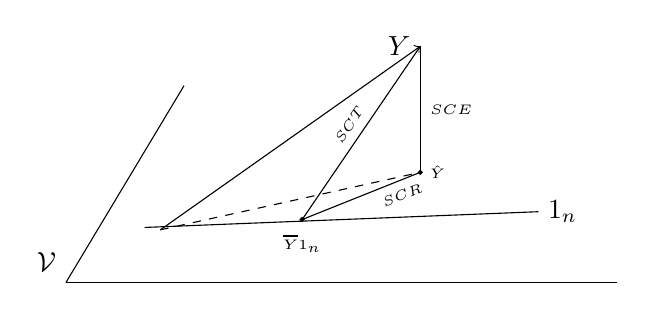
\begin{tikzpicture}
	% EV V
	\draw (0,-0.5) -- (1.5,2);
	\draw (0,-0.5) -- (7,-0.5);
	\node [below left] at (0,0) {$\mathcal{V}$};
	% 1_n
	\draw (1,0.2) -- (6,0.4);
	\node [right] at (6,0.4) {$1_n$};
	% Y
	\draw[->] (1.2,0.17) -- (4.5,2.5);
	\node [left] at (4.5,2.5) {$Y$};
	% SCT
	\draw (3,0.3) -- (4.5,2.5) node [midway, above, sloped] (TextNode) {\tiny $SCT$};
	% SCR
	\draw (3,0.3) -- (4.5,0.9) node [pos=0.8, below, sloped] (TextNode) {\tiny $SCR$};
	% \overline{Y}·1_n
	\draw[fill] (3,0.3) circle [radius=0.025]; 
	\node at (3,0) {\tiny $\overline{Y}1_n$};
	% \hat{Y}
	\draw[fill] (4.5,0.9) circle [radius=0.025]; 
	\node[right] at (4.5,0.9) {\tiny $\hat{Y}$};
	% SCE
	\draw (4.5,0.9) -- (4.5,2.5) node [pos=0.5, right] (TextNode) {\tiny $SCE$};

	\draw[dashed] (1.2,0.17) -- (4.5,0.9);


\end{tikzpicture}